% Created 2019-11-28 Thu 11:08
% Intended LaTeX compiler: pdflatex
\documentclass[11pt]{article}
\usepackage[utf8]{inputenc}
\usepackage[T1]{fontenc}
\usepackage{graphicx}
\usepackage{grffile}
\usepackage{longtable}
\usepackage{wrapfig}
\usepackage{rotating}
\usepackage[normalem]{ulem}
\usepackage{amsmath}
\usepackage{textcomp}
\usepackage{amssymb}
\usepackage{capt-of}
\usepackage{hyperref}
\usepackage{minted}
\usepackage[margin=0.75in]{geometry}
\renewcommand{\familydefault}{\sfdefault}
\usepackage{xcolor}
\usepackage{fancyhdr}
\pagestyle{fancyplain}
\chead{Assignment 4 - Practical Statistics with R}
\lhead{Guilherme G. Haetinger}
\rhead{Fall 2019}
\usemintedstyle{friendly}
\author{Guilherme Gomes Haetinger}
\date{\today}
\title{Assignment 5}
\hypersetup{
 pdfauthor={Guilherme Gomes Haetinger},
 pdftitle={Assignment 5},
 pdfkeywords={},
 pdfsubject={},
 pdfcreator={Emacs 27.0.50 (Org mode 9.2.6)}, 
 pdflang={English}}
\begin{document}

\maketitle
\thispagestyle{empty}


\section{\underline{Data Observations}}
\label{sec:org8033d7f}

Let's, firstly, load the dataset and check its structure:

\begin{minted}[,bgcolor=lightgray]{r}
data <- read.csv("titanic3.csv")
str(data)
\end{minted}

\begin{verbatim}

'data.frame':	1309 obs. of  14 variables:
 $ pclass   : int  1 1 1 1 1 1 1 1 1 1 ...
 $ survived : int  1 1 0 0 0 1 1 0 1 0 ...
 $ name     : Factor w/ 1307 levels "Abbing, Mr. Anthony",..: 22 24 25 26 27 31 46 47 51 55 ...
 $ sex      : Factor w/ 2 levels "female","male": 1 2 1 2 1 2 1 2 1 2 ...
 $ age      : num  29 0.92 2 30 25 48 63 39 53 71 ...
 $ sibsp    : int  0 1 1 1 1 0 1 0 2 0 ...
 $ parch    : int  0 2 2 2 2 0 0 0 0 0 ...
 $ ticket   : Factor w/ 929 levels "110152","110413",..: 188 50 50 50 50 125 93 16 77 826 ...
 $ fare     : num  211 152 152 152 152 ...
 $ cabin    : Factor w/ 187 levels "","A10","A11",..: 45 81 81 81 81 151 147 17 63 1 ...
 $ embarked : Factor w/ 4 levels "","C","Q","S": 4 4 4 4 4 4 4 4 4 2 ...
 $ boat     : Factor w/ 28 levels "","1","10","11",..: 13 4 1 1 1 14 3 1 28 1 ...
 $ body     : int  NA NA NA 135 NA NA NA NA NA 22 ...
 $ home.dest: Factor w/ 370 levels "","?Havana, Cuba",..: 310 232 232 232 232 238 163 25 23 230 ...
\end{verbatim}

We see the factor of sex and whether it survived or not. Let's check the correlation of those variables as they are displayed in the dataset. We can create a graph as follows:

\begin{minted}[,bgcolor=lightgray]{r}
survivorsData <- data %>%
      group_by(sex) %>%
      summarize(meanSurvivors = mean(survived))

survivorsData %>%
      ggplot(aes(sex, meanSurvivors, fill = "orange")) +
      geom_bar(stat="identity") +
      guides(fill=FALSE)
\end{minted}

\begin{center}
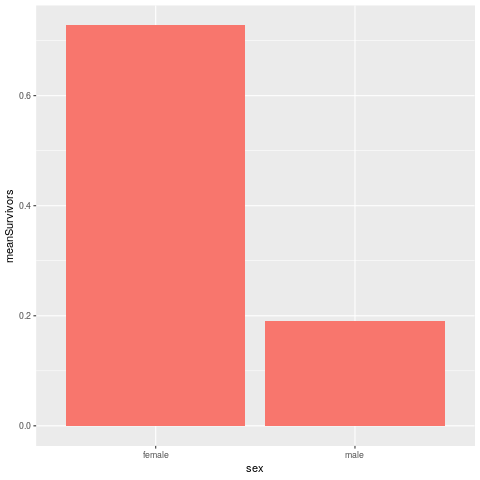
\includegraphics[width=.9\linewidth]{simpleCorrelation.png}
\end{center}

\begin{minted}[,bgcolor=lightgray]{r}
obs_diff <- abs(diff(survivorsData$meanSurvivors))
obs_diff
\end{minted}

\begin{verbatim}
0.536483232273864
\end{verbatim}


Taking this into consideration, it would seem that \textbf{sex} is a variable that influences whether someone will survive or not. To check if this represents the truth, we use randomization to create replicates.  

\section{\underline{Inference Structure}}
\label{sec:orgda2420c}

For this scenario, we have to consider the following:

\begin{itemize}
\item \colorbox{yellow}{Null Hypothesis} \(\to\) The sex has no influence whatsoever in whether the person survives or not.

\item \colorbox{yellow}{Alternative Hypothesis} \(\to\) The probability of not surviving while being a woman is higher than the probability of the same event while being a man.
\end{itemize}

By looking at the graph plotted in the previous section, we have that \(diff_{null} = 0.536\). In the following section, let's try creating random replicates to check our alternative hypothesis.

\section{\underline{Randomization}}
\label{sec:org2262463}

The replicate creation goes as follows:

\begin{minted}[,bgcolor=lightgray]{r}
new_data <- data %>%
      mutate(stringSurv = case_when(survived == 1 ~ "survived",
                                    survived == 0 ~ "died"))

replicates <- new_data %>%
  specify(stringSurv ~ sex, success = "survived") %>%
  hypothesize(null = "independence") %>%
  generate(1000, type = "permute") %>%
  calculate(stat = "diff in props", order = c("male", "female"))
\end{minted}

\begin{minted}[,bgcolor=lightgray]{r}
replicates %>%
  ggplot(aes(stat)) +
  geom_histogram(binwidth = 0.001) +
  geom_vline(aes(xintercept = obs_diff), color = "red")
\end{minted}

\begin{center}
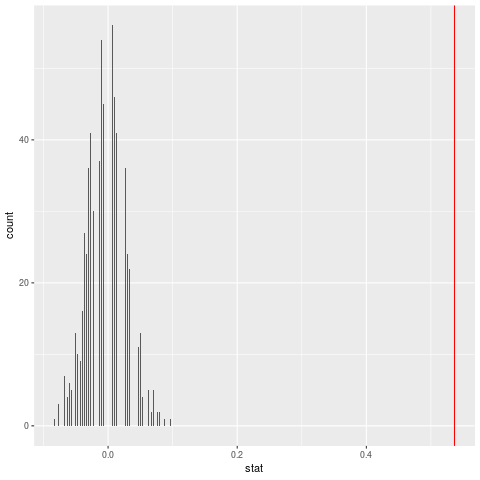
\includegraphics[width=.9\linewidth]{replicates_comparison.png}
\end{center}


As we can see, the difference calculated between the replicates never gets to the original difference. This means that the original distribution is unusual and it's highly unlikely that the value of \textbf{sex} has anything to do with the outcome of \textbf{survived}.
\end{document}
